\documentclass[letterpaper, 10 pt, conference]{ieeeconf}  % Comment this line out if you need a4paper

%\documentclass[a4paper, 10pt, conference]{ieeeconf}      % Use this line for a4 paper

\IEEEoverridecommandlockouts                              % This command is only needed if 
                                                          % you want to use the \thanks command

\overrideIEEEmargins                                      % Needed to meet printer requirements.

%In case you encounter the following error:
%Error 1010 The PDF file may be corrupt (unable to open PDF file) OR
%Error 1000 An error occurred while parsing a contents stream. Unable to analyze the PDF file.
%This is a known problem with pdfLaTeX conversion filter. The file cannot be opened with acrobat reader
%Please use one of the alternatives below to circumvent this error by uncommenting one or the other
%\pdfobjcompresslevel=0
%\pdfminorversion=4

% See the \addtolength command later in the file to balance the column lengths
% on the last page of the document

% The following packages can be found on http:\\www.ctan.org
\usepackage{graphics} % for pdf, bitmapped graphics files
\usepackage{epsfig} % for postscript graphics files
\usepackage{mathptmx} % assumes new font selection scheme installed
\usepackage{times} % assumes new font selection scheme installed
\usepackage{amsmath} % assumes amsmath package installed
\usepackage{amssymb}  % assumes amsmath package installed

\title{\LARGE \bf
Fundamental Diagram in the Shared Space enviroment Computer Simulation
}

\author{Tomoki Osaki$^{1}$ and Bernard D. Researcher$^{2}$
\thanks{*This work was not supported by any organization}% <-this % stops a space
\thanks{$^{1}$Tomoki Osaki is with Graduate School of Informatics,
        Nagoya University, Furo-cho, Chikusa-ku, Nagoya, Aichi, Japan
        {\tt\small tomoki.osaki.x5@s.mail.nagoya-u.ac.jp}}%
\thanks{$^{2}$Bernard D. Researcheris with the Department of Electrical Engineering, Wright State University,
        Dayton, OH 45435, USA
        {\tt\small b.d.researcher@ieee.org}}%
}

\begin{document}

\maketitle
\thispagestyle{empty}
\pagestyle{empty}


%%%%%%%%%%%%%%%%%%%%%%%%%%%%%%%%%%%%%%%%%%%%%%%%%%%%%%%%%%%%%%%%%%%%%%%%%%%%%%%%
\begin{abstract}
This electronic document is a live template. 
\end{abstract}
%%%%%%%%%%%%%%%%%%%%%%%%%%%%%%%%%%%%%%%%%%%%%%%%%%%%%%%%%%%%%%%%%%%%%%%%%%%%%%%%

\section{INTRODUCTION}
\subsection{Shared Space and Movement Efficiency}
In recent years, shared space, which is a kind of urban design has been increasingly introduced especially in some Europian urban areas. Compared to the conventional separated road, in shapred space, all road users (e.g., pedestrians, bicycles, and cars) use the same space. Additionally, at the intercations of those road users, who has the priority is ambiguous. Thus far, the study of collision avoidance has been conducted in the context of merging at the heighway or etc, however, the situation in the shapred space is far different from the situaion that previous studies have assumed.

\subsection{Traffic Flow in Traditional Road}
In the traditional traffic, the fundamental diagram theory has been proposed as the mechanism of traffic jam.

\begin{figure}[thpb]
   \centering
   \framebox{\parbox{3in}{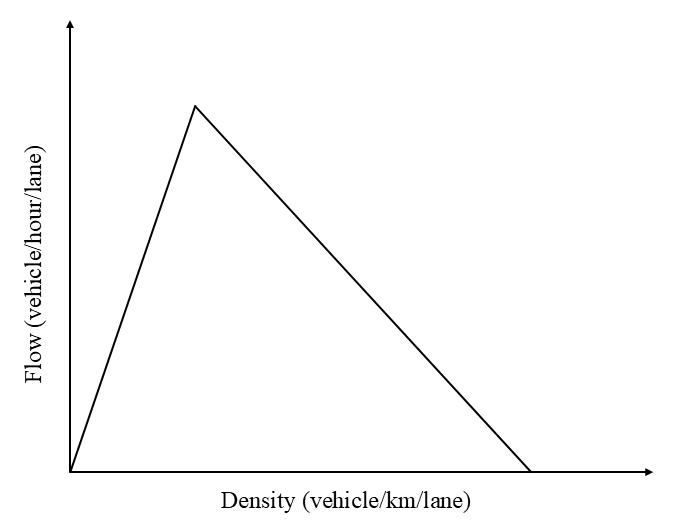
\includegraphics[scale=0.4]{figs/triangular_FD.png}}}
   \caption{The triangular relationships between the traffic density and the traffic flow.}
   \label{fig:triangular_fd}
\end{figure}

\subsection{Braking Index}
In a shared space, collision avoidane models developed by the previous studies might not be efficient because various road users coexist and there are no explicit rules for the priority. To address this problem, Matsubayashi et al. developed the braking index, which refers how many people brake at a certain timing to avoid a collision \cite{c2}. The braking index is given by the following equation (1).

$$
p = \frac{1}{1 + e^{-(a+b \cdot DCPA)}} \times \frac{1}{1 + e^{-(c+d \cdot TCPA)}} \eqno{(1)}
$$

\section{OBJECTIVE}
This study examined how the whole movements efficieny would change as the ratio of agents whose movement algorithms are different. We expected to find the threshold of the ratios of agents in the whole space that drastically change the movement effciiency. For example, considering the experiment carried by \cite{c2}, one qurater of whole agents could be one of the bottleneck; namely, when the number of cooperative agents reached the one qurater of the whole agents, movement efficiency drastically increased. Otherwise, there is also possibility that the raise of movement efficiency follows the linear change and the movement efficiency and the ratio of cooperative agents are in proportion. 

\section{METHOD}
To achive the objective of the study, we performed the computer simulation and measured the changes of fluency of movements as the number of agents increases.  

\subsection{Simulation Environment}
The space of the simulation environment was set as a 500 by 500 pixel virtual space, where the simulation agents could move in two dimensions. Thus, the simulation environment was made to represent the shared space (Figure \ref{fig:sim_env}). The space was designed as a torus so that when agents exceed any boundaries of the space, the agent was reallocated at the opposite positions to where the agent was before reallocation. The size of each agent was defiend as the radius of 5 pixel circle. Simulation finished when agents moved 500 times. All agnets' initial positions and initial velocities were randomized each time the simulation started. All agents' goals were set as the positions where each agents would pass through when kee

\begin{figure}[thpb]
   \centering
   \framebox{\parbox{3in}{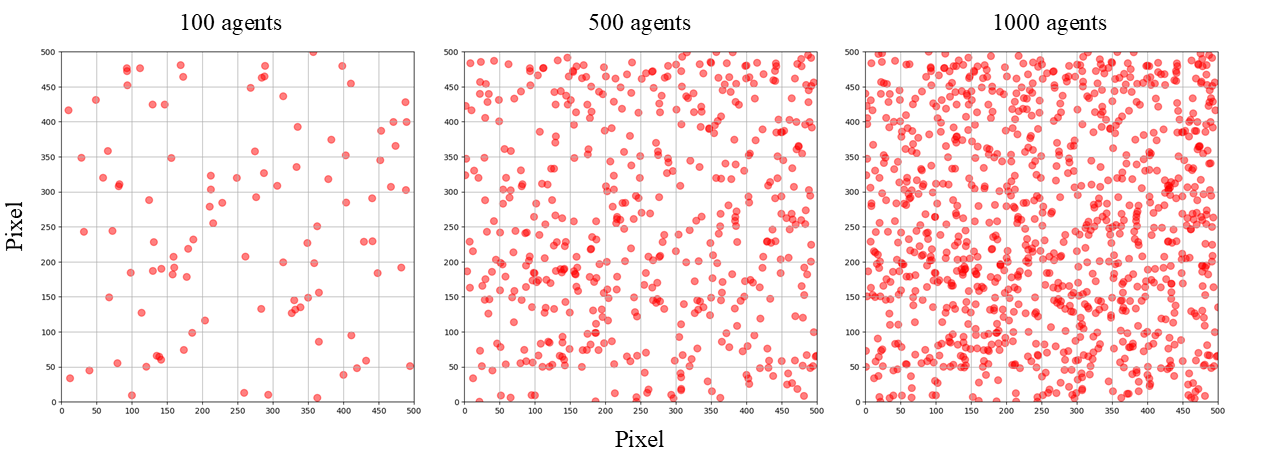
\includegraphics[scale=0.22]{figs/overview_simulation.png}}}
   \caption{The simulation environments with different number of agents.}
   \label{fig:sim_env}
\end{figure}


\subsection{Collision Avoidance Algorithms}
There were two types of collision avoidance algorithm. 

For one of types, simple avoidance, their avoindace vectors were generated to the opposite direction of the other agents which approached within a 50 pixel. The size of avoidance vectors were fixed as either 2, 3, or 4 pixel in one trial. We call this type of agents as the simple avoidance agents.

For another type of agent, which we call as the dynamic avoidance agent, their avoidance vector were generated based on the braking index. When an agent approch to another agent within 50 pixel, the braking index was calculated based on their relative positions and velocities, and their avoidance vectors were determined from 1 to 3 pixel. This way of avoidance enabled agents to avoid other agents considering how much potential danger they are facing; in safer situations, agents avoid slightly, on the contrary, in more dangerous situation, agents avoid widely. 

All agents always have 3 px goal directed vector and their moving vector were the composition of the goal directed vector and the avoidance vector. 

\subsection{Variables to evaluate the performance}
To evaluate the performance, we changed the number of agents and measured the total goal count of all agents and the number of collisions. The number of agents was changed from 100 to 1000 by 100.  Number of collisions is the mean of how many times each agent collided with other agents. When more than two agents approached each other at the distance of closer than 5 pixel, those agents' collision count was added. 


\section{RESULTS} 
Figure \ref{fig:result1} shows the results of the simulation. X axis refers to the number of the agents. The left Y axis refers to the total goal counts of all agents, and the right Y axis refers to the number of collisions.  

\subsection{Number of agents and the total goal counts}
First of all, line graphs show that, regradless of the types of collision avoidance algorithms, the relationships between the number of agents and the total goal count are similar to the triangular FD, i.e., to a certain amount of agents, total goal counts increase, however, after reaching the maximum goal counts, additional increasing of agents will conversely decreases the total goal counts. 

\subsection{Number of agents and the collisions}
Considering that the comfortably movable enviroment should be achieved not only by traffic smoothness but also by safety, we next focus on the bar graph representing the number of collisions. When looking at the bar graphs, dynamic avoidance algorithms made the least collisions. Comparing only among simple avoidance algorithms, simple avoidance 2 px, which avoid slightly made the least collisions, but from 700 agents, the number of collisions of simple avoidance 3 and 4 px become more than simple avoidance 2 px.

\begin{figure}[thpb]
   \centering
   \framebox{\parbox{3in}{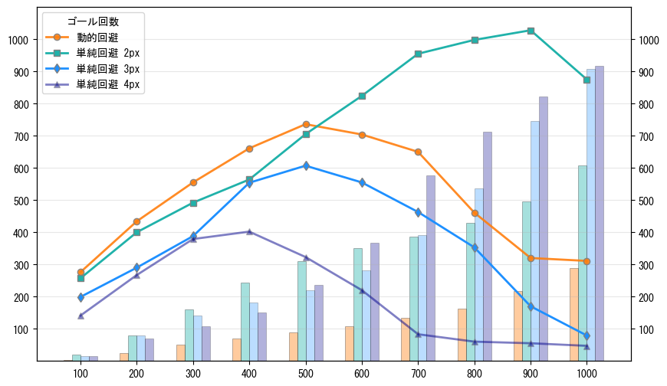
\includegraphics[scale=0.45]{figs/result1.png}}}
   \caption{The transitions of the total goal count of all agents and the number of collisions as the agents increases.}
   \label{fig:result1}
\end{figure}

% place the figure at the center ignoring columns
%\begin{figure}[t]
%   \begin{center}
%      \framebox{{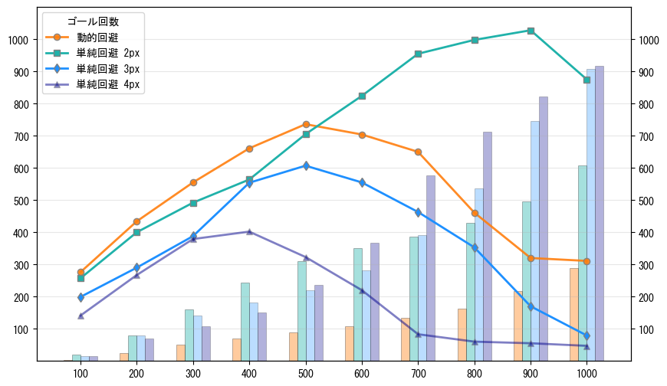
\includegraphics[scale=0.7]{figs/result1.png}}}
%      \caption{The transitions of the total goal count of all agents and the number of collisions as the agents increases.}
%      \label{fig:result1}
%   \end{center}
%\end{figure}

\section{DISCUSSION}
As the results showed, simualtions revealed that there is a triangular relationships between the number of agents and the total goal counts. This result implies that the traditional fundamental diagram theory might be applied to two-dimensional traffic environment. Additionally, the results also showed that dynamic avoidance algorithm, which was developed reflecting people's risk perception, made less collisions to other avoidance algorithm, which generates avoidance vector of fixed magnitude. Surprisingly, in all different number of agents environment, dynamic avoidance agents made less collisions than the simple avoidance 4 px, which always makes agents avoid more significantly than the dynamic avoidance. This result shows the probability that implementing the braking index to the mobility control might improve the safety of automatic driving, rather than using rule based collision avoidance algorithm. 

\section{CONCLUSIONS}
This study supplied the following two remarkable results.

\begin{itemize}
\item The relationships between the number of agents and the total goal counts in the shared-space environement could be approximated as the triangular fundamental diagram.
\item The collision avoidance algorithm based on people's risk perception could achive more safe movements in the shared-space enviroment.
\end{itemize}

For the first finding, 

\addtolength{\textheight}{-12cm}  

\section*{APPENDIX}
Appendixes should appear before the acknowledgment.

\section*{ACKNOWLEDGMENT}
The preferred spelling of the word on the first page. 

\begin{thebibliography}{99}

\bibitem{c1} G. O. Young, Synthetic structure of industrial plastics (Book style with paper title and editor), in Plastics, 2nd ed. vol. 3, J. Peters, Ed.  New York: McGraw-Hill, 1964, pp. 1564.
\bibitem{c2} Matsubayashi, S., Miwa, K., Terai, H., and Ninomiya, Y. (2024). Index of braking behaviour in two dimensions within risk perception. Transportation research part F: traffic psychology and behaviour, 102, 164-176.

\end{thebibliography}

\end{document}
